\RequirePackage{luatex85}
\documentclass[border=1mm]{standalone}
\usepackage{myFig}
\begin{document}
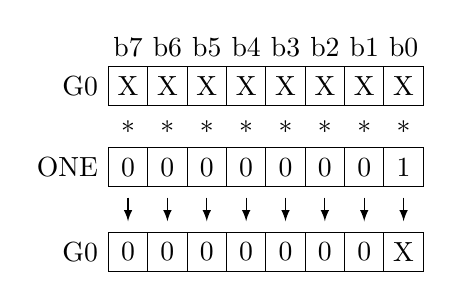
\begin{tikzpicture}[x=5mm, y=5mm]
  \tikzstyle{fixed}=[anchor=north, minimum width=5mm, minimum height=5mm]
  \foreach \x in {0,1,...,7}{
    \node (b\x) at (7-\x, 0) {b\x};
    \node[fixed, draw] (c\x) at (b\x.south) {};
    \node[fixed] (d\x) at (c\x.south) {$\ast$};
    \node[fixed, draw] (e\x) at (d\x.south) {};
    \node[fixed] (f\x) at (e\x.south) {\tikz \draw[-latex] (0,0) -- (0,-3mm);};
    \node[fixed, draw] (g\x) at (f\x.south) {};
  }
  \foreach \y [count=\x from 0] in {X,X,X,X,X,X,X,X}
  \node at (c\x) {\y};
  \foreach \y [count=\x from 0] in {1,0,0,0,0,0,0,0}
  \node at (e\x) {\y};
  \foreach \y [count=\x from 0] in {X,0,0,0,0,0,0,0}
  \node at (g\x) {\y};
  \node[anchor=east, align=left] at (c7.west) {G0};
  \node[anchor=east, align=left] at (e7.west) {ONE};
  \node[anchor=east, align=left] at (g7.west) {G0};
\end{tikzpicture}
\end{document}
